\documentclass{article}

% Put % before of what you want disabled

% Select what to do with todonotes:
% \usepackage[disable]{todonotes} % notes not showed
\usepackage[draft]{todonotes}   % notes showed


\usepackage{lmodern}
\usepackage[T1]{fontenc}
\usepackage{float}
\usepackage[spanish,activeacute]{babel}
\usepackage[utf8]{inputenc}
\usepackage{mathtools}
\usepackage[colorlinks=true]{hyperref}
\usepackage{synttree}
\usepackage{url}
\hypersetup{
    colorlinks=true,
    linkcolor=blue,
    filecolor=magenta,
    urlcolor=cyan,
}
\usepackage{graphicx}
\usepackage{amsmath}
\title{Diseño de gramática para la codificación semántica de partituras musicales basada en Humdrum}
\author{Jorge Marco Esteve}

\begin{document}
    \maketitle

    \section{Introducción}
    \subsection{Objetivos}
    Este trabajo pretende mostrar la realización del diseño de una gramática formal paso a paso para la codificación
    de partituras musicales las cuales estén basadas en Humdrum.
    Para ello se tratará de dar una base sobre el tema explicando que es y para qué sirve un compilador dando a entender
    la importancia de una gramática formal para este. Además, repasaremos las diferentes formas de representación musical
    que ha habido a lo largo de estos años y la utilidad que puede dar esta gramática en el futuro.
    \subsection{Requisitos}

    \subsection{Enfoque}



    \section{Contexto}
    \subsection{Historia}
    A lo largo de la historia se han diseñado multitud de máquinas y computadores con el fin de intentar mejorar o acelerar
    la precisión de los cálculos. Podríamos empezar por Charles Babbage\cite{babbage}, inventor de la Máquina Analítica en 1840 que era capaz
    de realizar cálculos programables con saltos condicionales y bucles, para aquel entonces esta máquina era lo más cercano
    a lo que conocemos hoy en día como un computador. Pero no es hasta 1936 donde Alan Turing formalizó la primera idea
    abstracta de un computador, donde una máquina lee y escribe ceros y unos de una cinta infinita, denominada actualmente
    como memoria, donde hay un conjunto finito de instrucciones elementales, al que hoy en día llamamos programa. La Máquina
    de Turing fue uno de los avances más importantes de la informática ya que esta podría considerarse como un autómata
    capaz de reconocer lenguajes formales. Los avances realizados por Turing provocó que en la década de 1940 hubiera una
    gran cantidad de desarrollo de máquinas de computación electronicas cada vez más rápidas y precisas.

    En 1945 John Von Neumann propuso una arquitectura en la que junta dos claves de los computadores: almacenamiento de un
    programa en memoria y un conjunto de instrcucciones de procesamiento. Pero no es hasta 1948 cuando se contruye el primer
    computador con esta arquitectora en Manchester capaz de hacer realizar saltos condicionales y direccionamiento indirecto.

    Con el tiempo los computadores y la forma de programar fue cambiando, mejorando en rendimiento y tamaño. Empezando con los
    computadores UNIVAC que fue la primera computadora comercial fabricada en Estados Unidos en 1951 con tarjetas
    perforables. Pero poco después aparecio el primer lenguaje de un nivel algo mas elevado que este código máquina, el
    ensamblador.

    \subsection{Ensamblador}

    Con el ensamblador, en lugar de escribir el código en binario, el programador tenía una serie de notaciones mnemotécnicas
    que simplificaban y mejoraba la notación anterior. Una forma de decirlo, era un lenguaje más legible que código máquina,
    más sencillo de implementar y con mayor facilidad de encontrar errores en el.

    Lo que el ensamblador trataba de hacer es una traducción de estas reglas mnemotécnicas(lenguaje ensamblador) a
    código máquina(código binario).
    \begin{figure}[H]
        \centering
        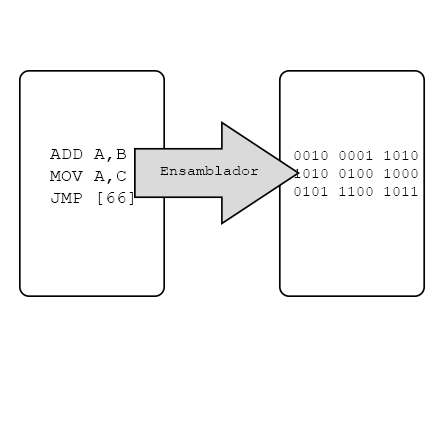
\includegraphics[scale = 0.6]{imagesMem/ensamblador.png}
        \caption{Proceso de ensamblador.}
    \end{figure}

    \section{Compiladores}
    Como hemos dicho un ensamblador, es un programa que se encarga de traducir el lenguaje ensamblador a código máquina.
    Con el paso del tiempo, se fueron desarrollando otros traductores de otros formatos de códigos/reglas que eran traducidos
    a ensamblador y este a su vez a código máquina.

    \begin{figure}[H]
        \centering
        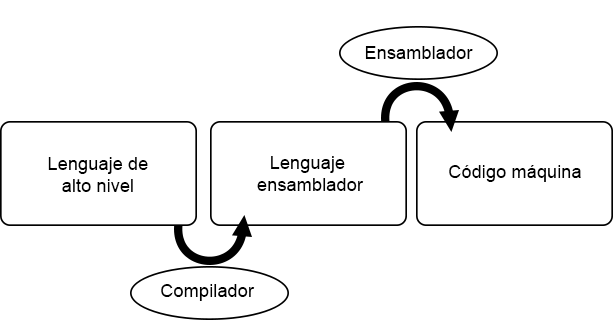
\includegraphics[0.8]{imagesMem/estrcompilador.png}
        \caption{Pasos de Lenguaje de alto nivel a código máquina.}
    \end{figure}


    Estos traductores de código de más alto nivel se denominaron compiladores. Estos lenguajes nos permiten una manera de
    programar más sencilla y dependiendo el lenguaje utilizado de una manera más detallada según el ámbito en el que queramos
    hacerlo. Una vez desarrollado el apartado de los compiladores, comenzaron a desarrollarse diferentes lenguajes. El primero
    de ellos fue FORTRAN en 1956, y lo siguieron muchos otros pasando por los principales de hoy en día como son C, C++,
    Java o Swift.

    Con el paso del tiempo los compiladores han sido desarrollados de manera más compleja, lo que ha provocado unos lenguajes
    con mejores prestaciones. Para poder traducir el código a ensamblador los compiladores cada vez deben realizar más tareas
    lo que produce que se hayan desarrollado las librerías, fragmentos de código escrito por otros programadores para simplificar
    la complejidad de lo que queremos implementar.

    \subsection{La compilación}
    Para lograr comprender las fases de la compilación, su recorrido y su finalidad debemos explicar previamente un término
    que hemos mencionado previamente en diversas ocasiones, qué es un lenguaje de programación.

    \subsubsection{Lenguaje de programación}
    Un lenguaje de programación es un lenguaje formal capaz de asimilar diferentes reglas conjuntas con el fin de poder
    controlar diferentes comportamientos de una computadora. Estos tienen sus propias ''palabras'' que las denominaremos \textit{tokens}
    y con la unión de estos \textit{tokens} rellenaremos las reglas que nos indicarán si el lenguaje en el que estamos programando
    está escrito de manera correcta o incorrecta. A este conjunto de reglas la llamaremos gramática, apartado donde nos
    centraremos más a fondo ya que es el tema principal de este trabajo.

    \subsubsection{Proceso de compilación}
    Como ya hemos explicado antes, un compilador es una herramienta que nos permite traducir un lenguaje de programación
    ''A'' a un lenguaje de programación ''B''. Para este proceso el compilador realiza diferentes procesos llegar al código
    de destino, como podría ser el lenguaje ensamblador para que este después sea ensamblado y traducido a código máquina,
    partiendo del código de inicio o código fuente como llamaremos a partir de ahora. Estos procesos hacen que el compilador
    pase una serie de normas para comprobar que el código esta correctamente escrito y no haya ningún tipo de errores, ya
    sean léxicos, sintácticos o semánticos. En la siguiente figura podemos observar un esquema del funcionamiento que realiza
    un compilador.

    \begin{figure}[H]
        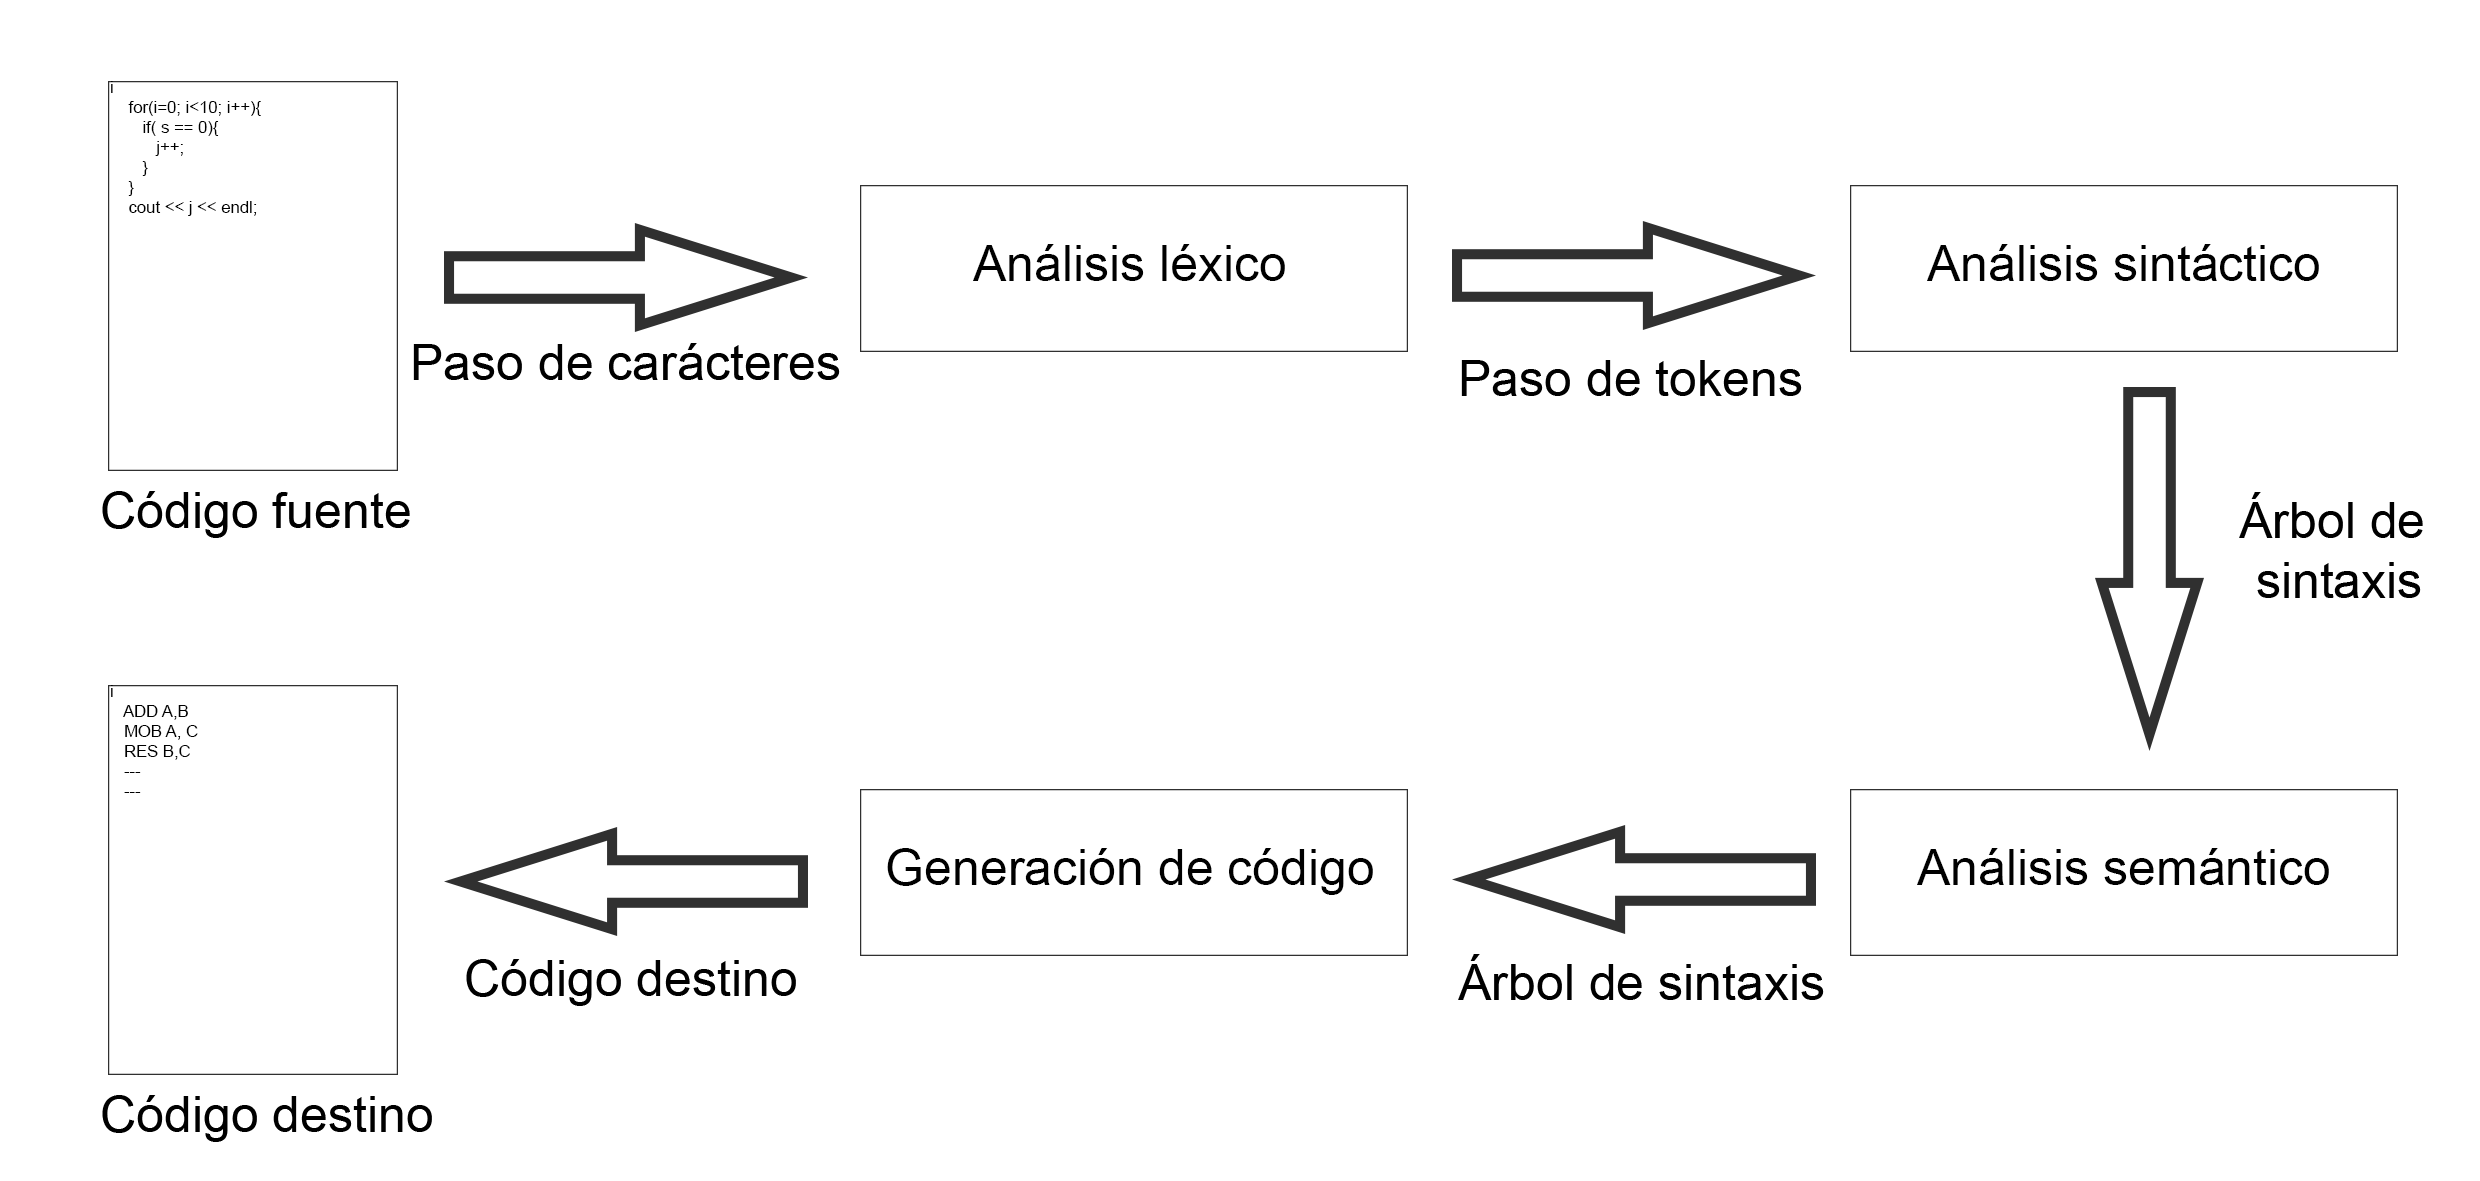
\includegraphics[scale = 0.55]{imagesMem/fasesCompilador.png}
        \caption{Estructura básica de un compilador}
    \end{figure}

    A simple vista en la imagen divisamos dos tipos de figuras, rectángulos y flechas, el primero corresponde la acción
    que se realiza en ese momento y la segunda el flujo de datos que vamos a enviar de una posición origen a una posición
    destino, donde el nodo inicial y final correspondera al código inicial y al código destino respectivamente. A continuación,
    pasamos a explicar cada una de partes de la imagen anterior.

    \subsubsection*{Código fuente}
    El código fuente es la información inicial que obtendrá el compilador para ser traducido que suele almacenarse en
    ficheros, ya puede ser uno o varios. Nuestro compilador tratará de leer dichos ficheros almacenando los caracteres en
    el computador y pasándolo a la siguiente acción.

    \subsubsection*{Análisis Léxico}
    El analizador léxico, respecto al compilador, es el único módulo que maneja el fichero de entrada o código fuente,
    se encarga de abastecer al analizador sintáctico una serie de unidades logicas denominadas \textit{tokens}
    o eleméntos lógicos que es el resultado de la agrupación de los caracteres previamente mencionados del código fuente.

    Éste suele ser una función o un método que es llamado por el analizador sintáctico cada vez que se necesitara conocer
    un nuevo \textit{token} para que el proceso de traducción siga.

    Existen diversidad de tipos de \textit{tokens} como puede ser:
    \begin{itemize}
        \item Palabras reservadas.
        Como es el caso de los diferentes códigos más famosos de programación como C o Java, hay palabras reservadas básicas
        como \textbf{if}, \textbf{else} que dan lugar a operaciónes lógicas.
        \item Símbolos especiales. Como puede ser \textbf{+} o \textbf{\&\&}, es decir, operadores aritméticos o lógicos entre
        otros
        \item Cadenas no específicas. Estos \textit{tokens} suelen ser \textbf{identificadores} o \textbf{números} entre otros que
        suelen ser utilizados para uso de variables internas del código.
    \end{itemize}

    Una cadena que ya ha sido reconocida como un \textit{token} específico es denominada como \textbf{lexema}, este no tiene un
    papel estructural, ya que esto se encargará de realizarlo el siguiente apartado, pero sí tiene un punto de vista semántico
    y nos servirá para identificar, si lo hay, cualquier tipo de error de escritura, ya que junto al \textit{token} almacenamos la
    fila y la columna en el que este se encuentra en el código fuente.

    Para identificar un \textit{token}, se deberá pasar carácter a carácter al analizador léxico el cual irá identificandolo por medio
    de un diagrama de transición previamente programado. Un diagrama de transición es la representación de los estados que puede
    tomar un sistema y muestra los eventos que implican un cambio a otro estado. Estos parten de un estado inicial y concluyen en uno final
    representado por nodos, el paso de un nodo a otro se realiza mediante eventos que los representaremos como aristas y le atribuiremos
    la acción de estos eventos.
    En la siguiente imagen tenemos sencillo ejemplo para lograr entenderlo.

    \begin{figure}[H]
        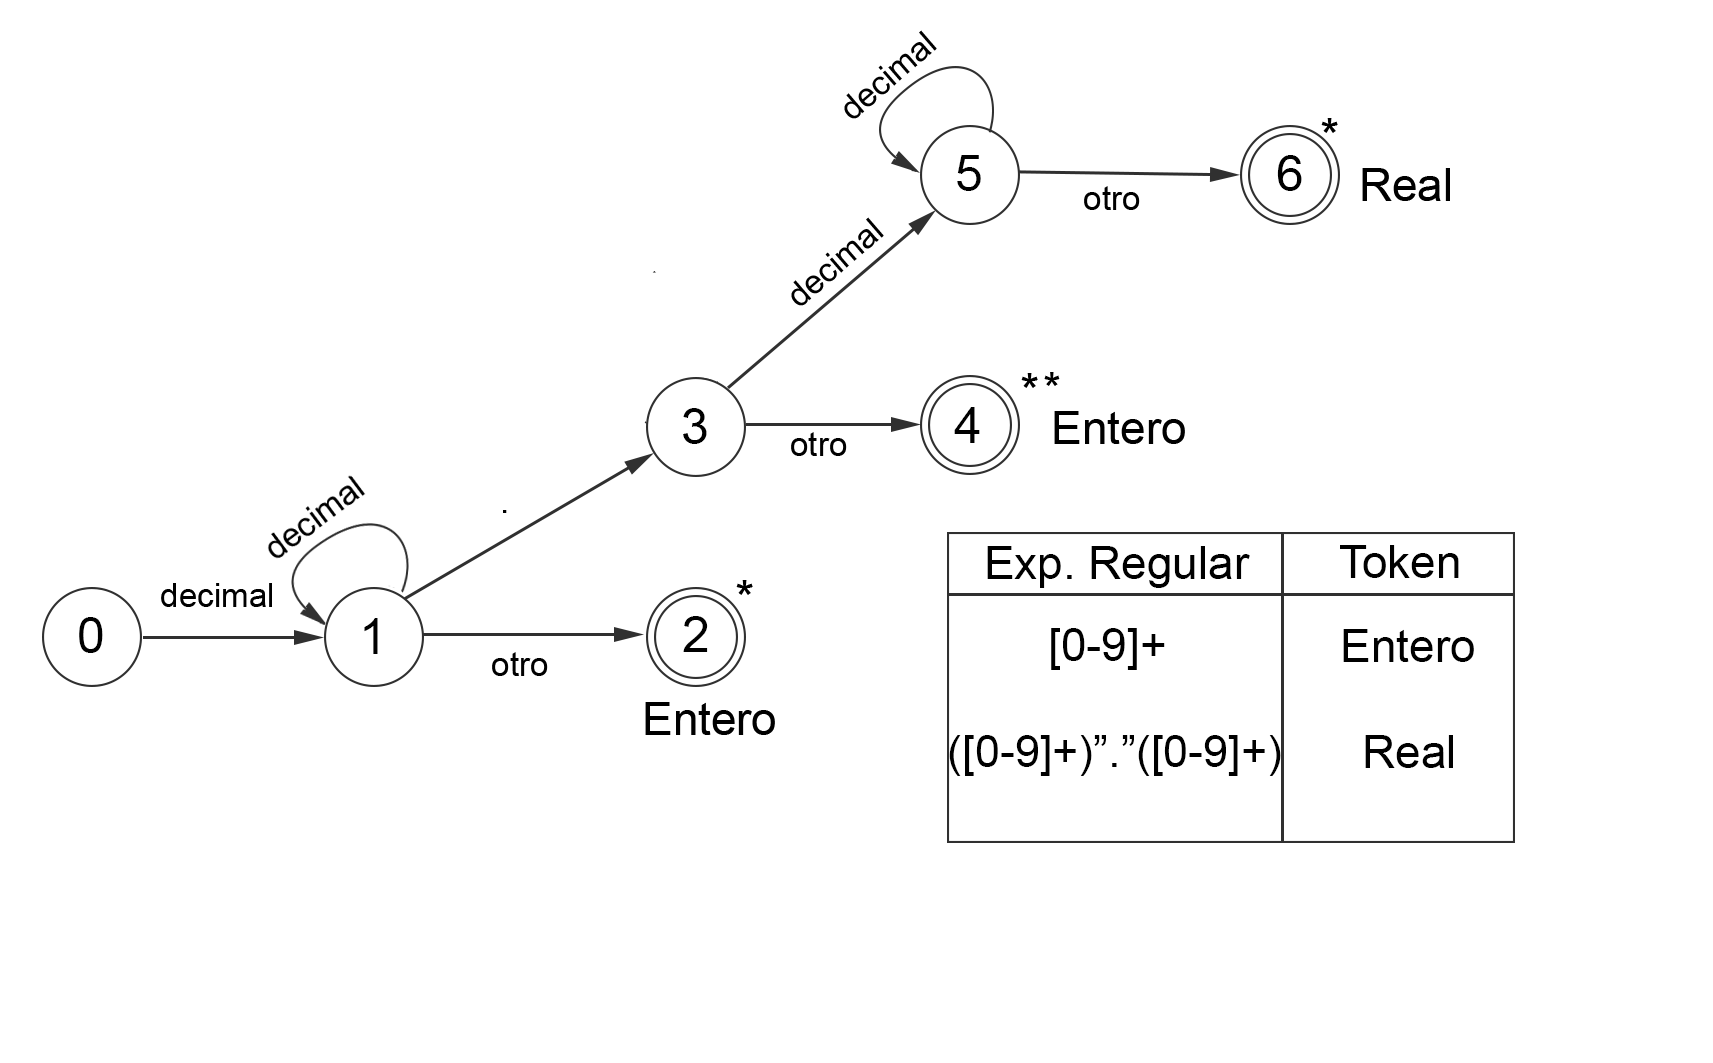
\includegraphics{imagesMem/diagramaTransicion.png}
        \caption{Ejemplo de diagrama de transición de un compilador donde se registran los números enteros y los reales}
    \end{figure}

    Dado el diagrama de transición, podemos implementar un programa (analizador léxico) capaz de identificar \textit{tokens} que
    corresponderan a números reales y números enteros, sabiendo que tendremos tres tipos de entradas correspondientes a
    \textbf{decimal} que serán los números del 0 al 9, el punto y cualquier otro valor que lo denominamos \textbf{otro}.

    Digamos que tenemos una traza, por ejempo \textit{1.2a} nuestro analizador cogería el primer caracter, el decimal 1
    y estaría en la posición 0 del diagrama, al ser un decimal, haríamos la transición a la posición 1 y cogeríamos el siguiente
    carácter, el \textbf{" ."}, al ser un punto la transición la haríamos a la posición 3 y no a la dos ya que para esta debería ser
    cualquier otro valor que no fuera un decimal o un punto. A continuación, analizaríamos el siguiente carácter, el 2, por
    el mismo método que antes pasaríamos a la posición 5 ya que para la 4 debería ser cualquier caracter tipo \textbf{otro}. Ya
    en el 5 leeriamos el último carácter que faltara, en nuestro caso \textbf{a}, al no ser tipo decimal ni punto correspondería
    a un carácter tipo ''otro'', lo que nos haría concluir el \textit{token}, como indica el doble circulo, retrocediendo un carácter,
    este es el significado del asterisco, y obteniendo un \textit{token} \textbf{REAL} bajo el lexema 1.2.

    Una vez reconocido todo los caracteres del código y pasados a \textit{tokens} pasaremos a la la acción del analizador sintáctico.

    \subsubsection*{Análisis sintáctico}
    Como hemos mencionado, el analizador sintáctico obtiene los \textit{tokens} previamente mencionados llamando al analizador
    léxico. Este irá leyendo dichos \textit{tokens} a la vez que genera la traducción para el código destino, comprobando que la
    sintaxis, es decir, la agrupación de los \textit{tokens} en el orden de entrada son correctos.

    En definitiva, el análisis sintáctico sirve para comprobar que el orden de los \textit{tokens} es el correcto, esta forma de
    comprobar que el código está escrito de manera correcta lo realiza por medio de lo que denominamos  \textbf{Gramatica
    Formal}.

    Una gramática formal (''G'') es una estructura que representa un conjunto finito de reglas que describen
    toda la secuencia de \textit{tokens} pertenecientes a un lenguaje específico \textit{L}.

    La estructura algebraica de una gramática está formada por los siguientes elementos o nodos, como denominaremos a partir
    de ahora:

    \textbf{G} = \{ \textit{NT, T, S, P} \}
    en el que:
    \begin{itemize}
        \item NT es un conjunto de nodos No Terminales.
        \item T es el conjunto de nodos Terminales.
        \item S es el símbolo o nodo inicial de la gramática.
        \item P es el conjunto de reglas de producción.
    \end{itemize}

    Esto quiere decir, dado un símbolo inicial \textbf{S}, el cual será un nodo no terminal, generará un número de reglas
    de producción \textbf{P} con nodos terminales \textbf{T} y nodos no terminales NT. Esos nodos no terminales a su vez derivarán otras reglas
    que al igual que S obtendremos más nodos terminales y no terminales, con una finalidad de obtener al final del árbol
    nodos terminales ya que estos no generan reglas.



    \begin{table}[H]
        \centering
        \begin{tabular}{p{5cm}}
            S \rightarrow T \textbf{ id } R \\
            T \rightarrow \textbf{int} \\
            R \rightarrow \textbf{coma id } R \\
            R \rightarrow \textbf{puntoycoma}
        \end{tabular}
        \caption{Gramática de una declaración de variables tipo entero.} \label{tab:gram1}

    \end{table}

    Este es un ejemplo de una gramática sencilla en la cual tenemos un nodo inicial, dos nodos no terminales y
    cuatro nodos terminales:

    \begin{itemize}
        \item Nodo inicial (S) = \{S\}
        \item Nodos no terminales (NT) =\{T, R\}
        \item Nodos terminales (T) =\{id, int, coma, puntoycoma\}
    \end{itemize}

    Esta gramática representaría la declaración de una o varias variables de tipo entero. Para explicar el funcionamiento
    de la gramática mejor, vamos a representar un ejemplo con un arbol lógico bajo el código de entrada:

    \texttt{int i, j;}

    \begin{figure}[H]
        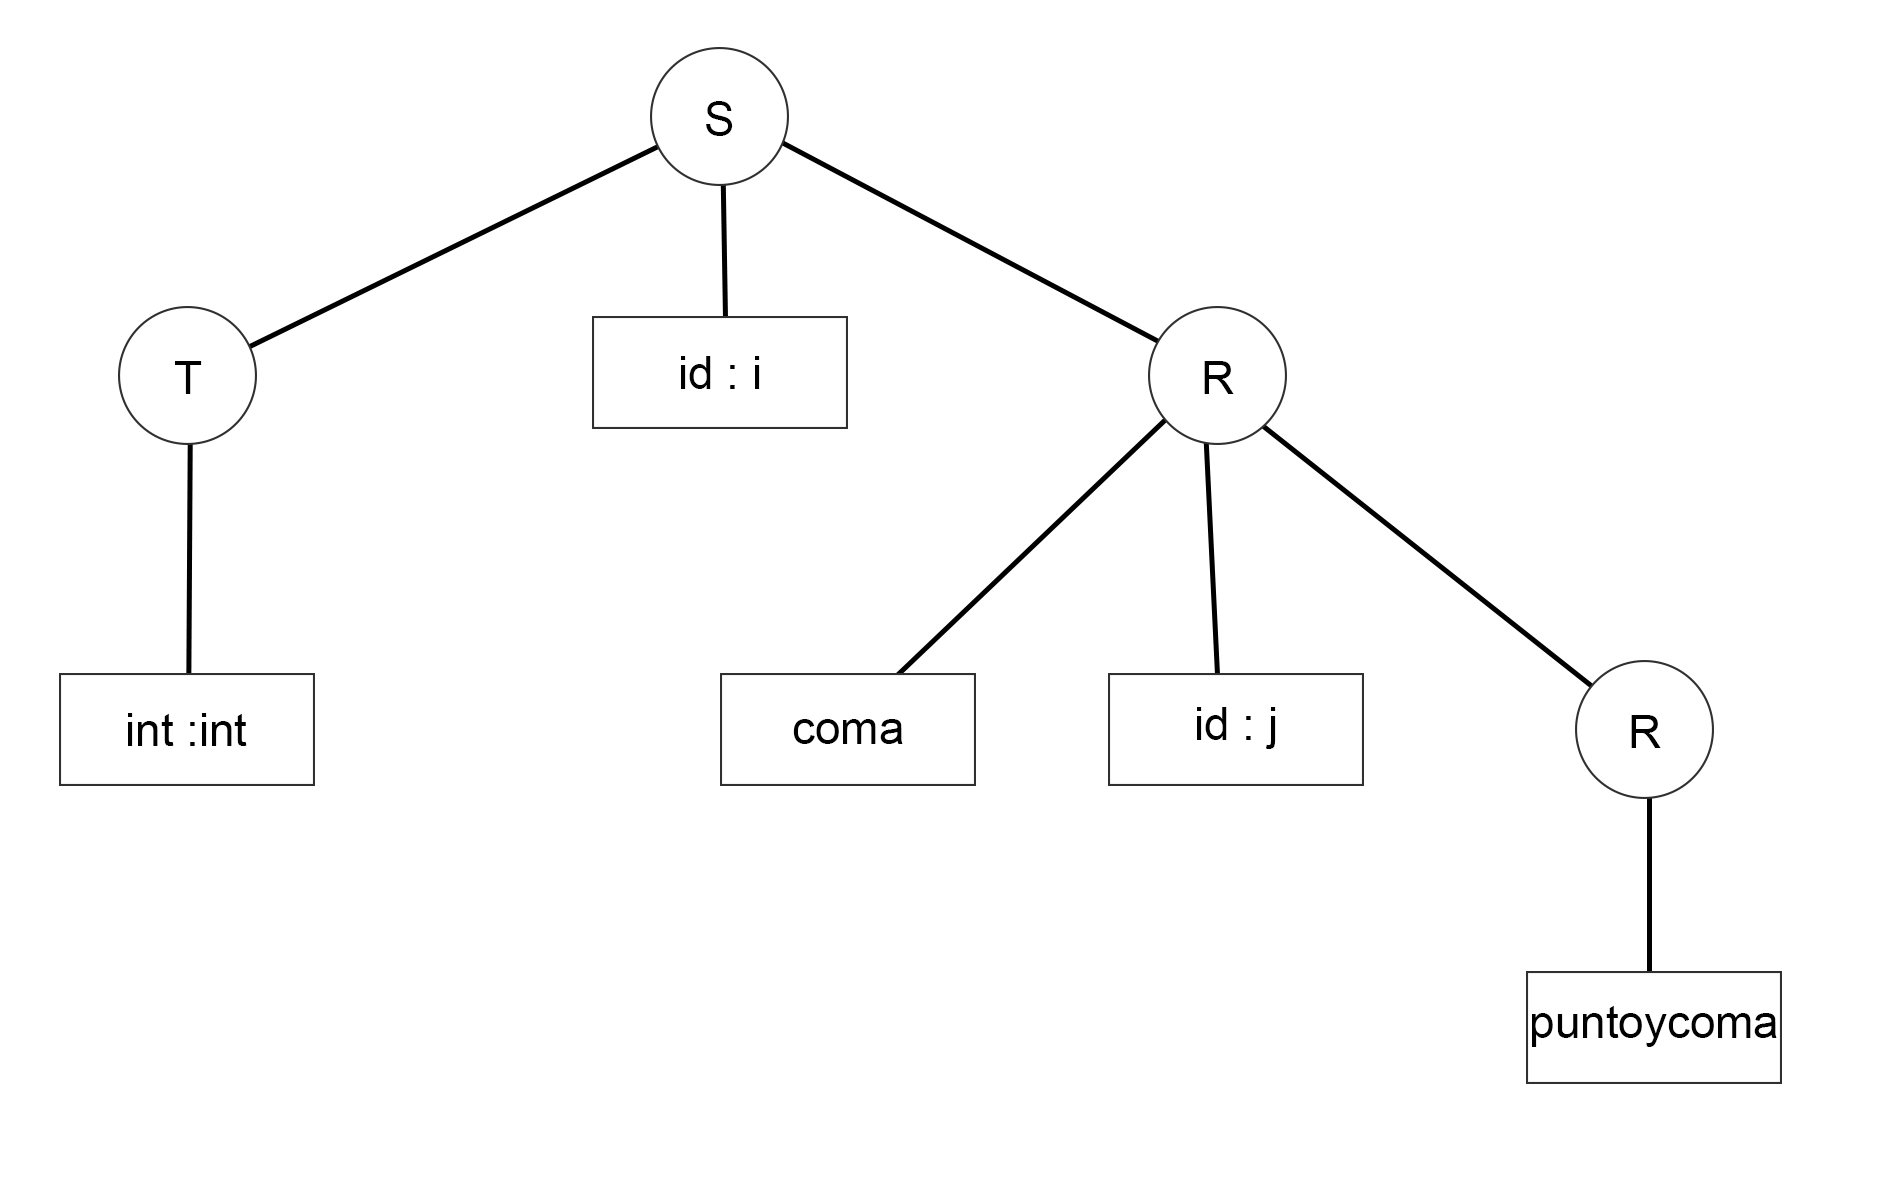
\includegraphics[scale = 0.7]{imagesMem/arbol.png}
        \caption{Árbol generado a partir del ejemplo para la gramática anterior.}
    \end{figure}


    En la figura anterior podemos observar un árbol lógico de decisiones representando el ejemplo previamente mencionado.
    En él podemos observar los nodos terminales y los nodos no terminales, representados respectivamente con rectángulos
    y círculos. Como vemos el nodo inicial o nodo raíz va derivando en otros nodos no terminales hasta llegar a la parte
    más baja de la ramificación con nodos terminales en los que, estos últimos, corresponderán a un tipo de \textit{token} expecifico.

    Una gramática libre de contexto, es una gramática formal en la que cada regla de producción está formada por un símbolo
    no terminal y una cadena de nodo terminales y/o no terminales.
    \begin{table}
        \centering
        \texttt{S \rightarrow w }
    \end{table}
    Se denomina de libre contexto porque el nodo no terminal \texttt{S} puede ser siempre sustituido por una cadena de caracteres
    \texttt{w} sin tener en cuenta el contexto en el que ocurra.
    Un problema que tiene el analizador sintáctico de una de estas gramáticas libre de contexto (\textit{Context-free grammar}),
    es su coste temporal ya que gira entorno a $O(n^3)$, que es demasiado alto. Para solucionar este problema y
    reducir su coste temporal a lineal, $O(n)$, existen dos
    estrategias que vamos a tratar a continuación:

    \begin{itemize}
        \item Análisis sintáctico descendente o ASD.
        \item Análisis sintáctico ascendente o ASA.
    \end{itemize}

    Estos tipos de analizadores pueden ser implementados a mano o usando generadores automáticos, ejemplos de este último
    son ANTLR y yacc/bison, los cuales hablaremos más adelane,mientras que la implementación a mano de estos analizadores
    son recomendables únicamente para gramáticas simples, ya que para una gramática muy compleja sería muy difícil de implementar.

    \subsubsection*{Análisis sintáctico descendente}

    Este tipo de análisis trata de reproducir la derivación por la izquierda de la cadena de entrada.
    respecto a nuestro ejemplo de gramática anterior, cuadro~\ref{tab:gram1}, quedaría de la siguiente manera:

    \begin{table}[H]
        \centering
        \begin{tabular}{p{0cm}p{5cm}}
            S & \rightarrow T \textbf{ id } R \\
            &  \rightarrow \textbf{int id(i) }  R \\
            &  \rightarrow \textbf{int id(i) coma id(j) } R \\
            &  \rightarrow \textbf{int id(i) coma id(j) } \textbf{puntoycoma}\\
        \end{tabular}
        \caption{Representación de análisis descendente}
    \end{table}

    En este caso podemos observar cómo desde un nodo inicial \textbf{S} se va derivando su regla y colocando los \textit{tokens}.
    Se le denomina análisis descendente porque comienza desde el nodo más alto del árbol y va descendiendo por los nodos
    no terminales hasta llegar a los nodos terminales y comprobando que la sintaxis está bien hecha.

    Para realizar bien el analizador sintáctico descendente la cadena de entrada debe encontrar por medio de las
    reglas de producción una representación de dichas reglas en el orden correcto. Para ello, la
    gramática no puede ser ambigua ni determinista, de tal forma que sólo debe existir un árbol de derivación posible para
    cada sentencia y para cada nodo que nos encontramos y con cualquier símbolo leido,
    siempre va a haber no más de una transición posible del nodo y con ese símbolo. Finalmente, no puede ser una gramática
    recursiva por la izquierda ya que entraríamos en bucle infinito al derivar, esto quiere decir que entraría en bucle infinito
    al expandir un nodo no terminal a su regla de producción.

    Los analizadores sintácticos descendentes, por un conjunto de gramática libre de contexto, las entradas son de izquierda
    a derecha y las contrucciones de derivaciones son por la izquierda de una sentencia los denominamos \textbf{analizador
    sintáctico LL}.

    Los analizadores $LL$ son llamados analizadores $LL(k)$ si necesit analizar un número de k \textit{tokens} cuando el analizador va hacia delante
    en la sentencia, es decir, si hubiera para una gramatica tal analizador y pudiera analizar el código sin vuelta atrás (\textit{Backtraking}),
    termino que se emplea en algoritmos para buscar el retroceso en un árbol lógico y encontrar la solución deseada,
    entonces esta gramática la denominaríamos gramática $LL(k)$. Las gramáticas más populares son las $LL(1)$ que a pesar
    de poder ser muy restrictivas sólo necesita ver el siguiente \textit{token} para hacer el análisis sintáctico.

    Una gramática cumple la condición $LL(1)$, si para todos los nodos no terminales, no existen símbolos comunes en los
    conjuntos de predicción de sus reglas. Los conjuntos de predicción ayudan a decidir que regla utilizar en cada paso.
    \todo[inline]{¿Debo explicar detalladamente los conjuntos de predicción con los primeros y los siguintes?}
    En un principio, debemos partir que una gramática es $LL(1)$ y a partir de ahí intentar negarlo, para ello debemos
    comprobar que no cumple con la condición $LL(1)$, pero además hay algunas características que hacen que una gramática
    no sea LL(1) que, de otra manera, las hemos mencionado anteriormente:

    \begin{itemize}
        \item Que tenga recursividad por la izquierda. $$ P  \rightarrow P \ \ldots $$
        $$ P \rightarrow \ \ldots $$
        \item Que tenga factores comunes por la izquierda.$$ P \rightarrow \alpha \  S_1 $$
        $$ \ldots $$
        $$ P \rightarrow \alpha \ S_2 $$
        \item Que haya ambiguedad.
        \begin{table}[H]
            \centering
            \begin{tabular}{p{5cm}}
                S \rightarrow S \textbf{ + } S \\
                S \rightarrow S \textbf{ - } S \\
                S \rightarrow \textbf{ numero } \\
            \end{tabular}
        \end{table}

        Esta gramática sería ambigua ya que podríamos representar de dos formas diferentes una misma entrada como vemos
        a continuacion con la cadena de entrada \texttt{1 + 1 - 1}:

        \begin{table}[H]
            \synttree[S [S [numero[1]]] [+] [S [S[numero[1]]] [-] [S[numero[1]]]]]
            & \synttree[S [S [S [numero[1]]] [+] [S[nuemero[1]]]][-][S[numero[1]]]]
            \caption{Ejemplo de gramática ambigua}
        \end{table}
    \end{itemize}


    Una vez explicado esto y viendo la siguiente figura podemos saber a que nos referimos con gramáticas $LL(1)$.
    \begin{figure}[H]
        \centering
        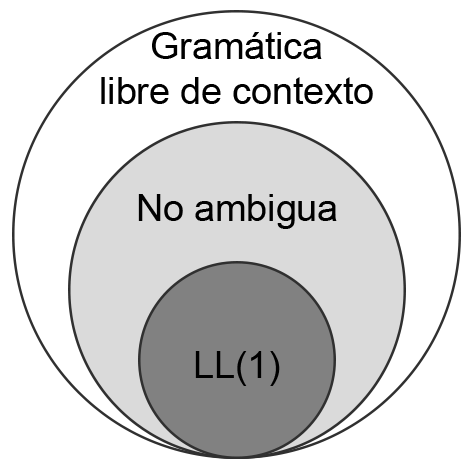
\includegraphics{imagesMem/LL1.png}
        \caption{Las gramáticas $LL(1)$ como subconjunto de las gramáticas libres de contexto y no ambiguas.}
    \end{figure}
    En definitiva, una gramática $LL(1)$ es una gramática la cual está libre de contexto y, además, no es ambigua.

    \subsubsection*{Análisis sintáctico ascendente}
    Los analizadores sintácticos ascendentes se le denominan de esta manera (en inglés \textit{botton-up}) porque su pretensión es
    la de construir un árbol sintáctico para una determinada cadena de entrada, empezando por sus nodos terminales y
    construyendo el árbol con sus nodos no terminales hasta llegar a la raíz o nodo inicial.
    También se le puede considerar a este proceso como la reducción de una cadena de símbolos al símbolo inicial de la
    gramática, es decir, una derivación en sentido inverso. Para detallar un poco más, en cada paso del proceso,
    una cadena que coincida con la parte derecha de la producción se reemplaza por el símbolo no terminal de la parte
    izquierda de la producción. A continuación vamos a observar un ejemplo de ello por medio de la gramática de el
    Cuadro~\ref{tab:gram1}:

    Para el ejemplo: \texttt{int i, j;}

    \begin{table}[H]
        \centering
        \begin{tabular}{p{7cm},p{0cm}}
             \textbf{\fcolorbox{black}{white}{int} id(i) coma id(j) puntoycoma} & \leftarrow \\
             \textcolor{red}{T} \textbf{ id(i) coma id(j) \fcolorbox{black}{white}{puntoycoma}} & \leftarrow \\
             T \textbf{ id(i) } \fcolorbox{black}{white}{\textbf{coma id(j) } \textcolor{red}{R}} & \leftarrow \\
             \fcolorbox{black}{white}{T \textbf{ id(i) } \textcolor{red}{R}} & \leftarrow \\
             \textcolor{red}{S}\\

        \end{tabular}
        \caption{Representación de análisis ascendente.}
    \end{table}

    En el ejemplo podemos ver que los símbolos encuadrados serán los que vamos a intentar simplificar a una regla, la cual
    en el siguiente paso la marcaremos de rojo, así paso tras paso hasta llegar al nodo raíz que nos verifique el correcto
    uso de la gramática.

    Este tipo de analizadores son de tipo reducción/desplazamiento, analizador LR, los cuales reconocen lenguajes realizando dos operaciones,
    cargar y reducir. Lo que hacen es leer los \textit{tokens} de la entrada e ir cargandolo en una pila, de forma que se puedan explorar
    los n \textit{tokens} que que contiene ésta y ver si se puede corresponder con la parte derecha de alguna de las reglas de la
    gramática. Si es así se realiza una reducción, la cual consiste en sacar de la pila esos n \textit{tokens} y en su lugar colocar
    el símbolo o nodo no terminal que le corresponde a esa regla. En caso contrario se carga en la pila el siguiente \textit{token}
    y una vez hecho esto se vuelve a intentar reducir hasta llegar al símbolo inicial de la gramática.

    Cabe mencionar que este tipo de analizadores deben saber identificar muy bien las reglas de producción para que no
    se quede bloqueado el análisis, ni tenga que hacer retroceso (\textit{backtracking}). Al igual que existen las gramáticas
    $LL(K)$ que hemos mencionado anteriormente, también están las gramáticas $LR(k)$ las cuales utilizan \textit{k} elementos
    léxicos(\textit{tokens}) de busqueda hacia delante.

    Estas gramáticas realizan eficientemente el análisis ascendente en el que no hay retroceso, ya que son reconocidas por
    un analizador $LR(k)$.
    Para construir un analizador de este tipo necesitamos un programa analizador LR, una tabla de análisis y una pila en
    los que se van cargando los estados que pasa el analizador y los símbolo de la gramática que se van leyendo.

    \subsubsection*{Análisis semántico}

    El análisis semántico del árbol de la sintaxis que recibimos empieza por detectar las incoherencias a nivel sintáctico
    en el propio árbol lo cual este análisis trata de generar los errores que el código fuente incorpora. Estos analizadores
    se les suelen denominar \textif{parsers}, los cuales buscan de una forma más concienzuda los \textit{tokens} que se generan del código
    inicial, y no puede ''gestionar'' el analizador sintáctico.

    \subsubsection*{Generación de código}
    Este apartado consiste en que, una vez comprobado que el árbol esta ordenado correctamente y que todos los \textit{tokens} tienen
    su lógica, el código es traducido por medio de sus \textit{tokens} en el cual tenemos su lexema, y que correspondera una traducción
    especifica, al código destino finalizando, de esta manera, el proceso de compilación habrá finalizado.


    \section{Intérpretes}
        Un intérprete es un programa que analiza y ejecuta simultáneamente un programa escrito en un lenguaje fuente.

    En la siguiente figura se representa lo que sería el esquema general de un intérprete, este lo podemos asemejar
    a una caja negra. En estos podemos identificar dos entradas: un programa \textbf{P} escrito en un lenguaje fuente \textbf{LF}
    junto con los datos de entrada. A partir de estos datos de entrada y mediante un proceso de interpretación se va produciendo
    unos resultados.

    \begin{figure}[H]
        \centering
        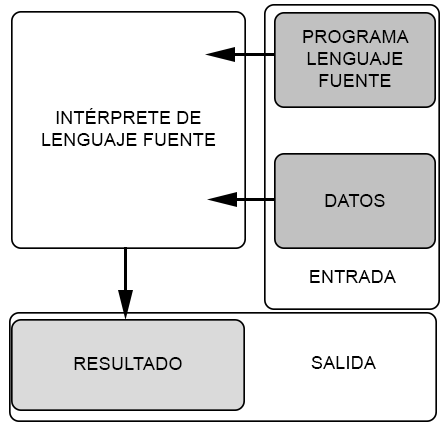
\includegraphics[scale = 0.6]{imagesMem/interprete.png}
        \caption{Estructura de un intérprete.}

    \end{figure}

    La diferencia entre compiladores e intérpretes es que los compiladores transforman el programa a un programa equivalente
    en un código diferente y éste es ejecutado dando los resultados en fase de ejecución.

    \subsection{Estructura de un intérprete}

    Cuando vamos a contruir un intérprete es conveniente utilizar una representación interna del lenguaje fuente a analizar.
    De esta manera, la organización interna de la mayoría de los intérpretes se descompone en varios modulos:

    \textbf{Conversión a representación interna}: La entrada del condigo del programa \texttt{P} en Lenguaje Fuente, es
    analizado y se transforma a la representación interna del programa \texttt{P}.

    \textbf{Representación interna}: Para crear esta representación se utilizan árboles sintácticos que obteniendo la traducción
    mediante una \textbf{Tabla de símbolos } se va rellenando con la traducción de estos símbolos de una manera ordenada
    y capaz de poder representar el lenguaje inicial.

    \textbf{Tabla de símbolos}: Durante el proceso de traducción, es conveniente ir creando una tabla con información
    relativa a los símbolos que aparecen. La información que almacenaremos en esta tabla será un conjunto de \texttt{tokens}
    en el que su complejidad residira en la complejidad del lenguaje inicial.

    \textbf{Evaluador de Representación Interna}: A partir de la implementación de la parte anterior se evaluan los datos
    de entrada y se lleva a cabo las acciones ne cesarias con el fin de obtener los resultados. Durante este proceso es
    necesario contemplar la aparición de errores.

    \textbf{Tratamiento de errores}: Durante la evaluación se pueden general diferentes errores que el intérprete debe
    contemplar, errores que no son capaces de contemplar en la parte de la representación interna.

    Dependiendo de la complejidad del código a analizar, el intérprete tiene la posibilidad de contener módulos similares
    a los del compilador tradicional: Análisis léxico, análisis sintáctico y análisis semántico.

    \subsection{Ventajas de los intérpretes.}

    En general, la utilización de compiladores permite contruir programas más eficientes que los correspondientes interpretados,
    ya que durante la ejecución de código compilado no es necesario realizar complejos análisis, además, un buen compilador es
    capaz de detectar errores y optimizar el código generado.

    Por otro lado, los intérpretes, proporcionan una mayor flexibilidad que permite modificar
    y ampliar las características del lenguaje fuente. Ejemplos como APL, Prolog o Lisp surgieron en primer lugar
    como sistemas interpretados y posteriormente surgieron compiladores.

    Facilitan la metaprogramación, programas que crean otros programas, lo cual ayuda a la programación de sistemas de
    aprendizaje automatizado.

    Debido a que no existen etapas intermedias de compilación, los sistemas interpretados facilitan el desarrollo rápido
    de prototipos, potencian la utilización de sistemas iteractivos y facilitan las tareas de corrección de errores.


    \section{Metaprogramas}

    Como ya hemos dicho anteriormente, hay dos formas de implementar analizadores, a mano, donde debes implementar tú mismo
    todas las funcionalidades de \textit{estos}, o usando generadores automáticos, como es el caso de ANTLR y Flex/Bison, las herramientas
    más utilizadas hoy en día para la creación de compiladores, los cuales,
    a partir de un conjunto de reglas, ellos mismos generan un analizador sintáctico, aunque de maneras diferentes que
    explicaremos a continuación.

    \subsubsection{Flex\cite{flex} y Bison\cite{bison}}

    En el caso de Flex y Bison, creados por Vern Parxson y Robert Corbett respectivamente, son dos herramientas en las que,
    la primera trata el léxico de la gramática produciendo los \textit{tokens} y pasándoselo al segundo que es el que crea el analizador
    sintáctico. Éste crea un analizador LALR, que es una mejora de los analizadores tipo LR(1). Como hemos explocado anteriormente,
    este tipo de analizadores sintácticos son ascendentes, los cuales generan los árboles de la sintaxis de abajo hacia arriba
    (down-top).

    \subsubsection{ANTLR}

    ANTLR\cite{antlr4} es un software desarrollado en \textit{Java} por Terence Parr, que implementa de una manera eficiente analizadores LL(k),
    esto quiere decir que el analizador sintáctico generado por ANTLR es descendente (top-down), creando el árbol sintáctico
    de arriba a abajo, es decir, desde el nodo inicial de la gramática y los no terminales. Además es capaz de generar el
    análisis lexico y el propio código destino, por medio del análisis semántico y traduciéndolo. En pocas palabras, puede
    realizar todas las fases de un compilador, pasándole una gramática e implementando los \textit{parsers} y las traducciones
    necesarias. Más adelante concretaremos otros aspectos que recoje esta herramienta.



    \section{Gramática para Kern\cite{kern} y Mens\cite{mens}}
    Como hemos dicho al inicio la creación de nuestro trabajo se va a basar en la creación de una gramática formal en la
    que podamos representar el lenguaje musical. Para ello necesitamos, también, entrar un poco en contexto sobre la representación
    musical.
    \subsection{Representación musical}
    Los códigos musicales han sido utilizado desde sus inicios para facilitar la transcripción de sonidos, desde los neumas
    que se representaban el canto en monasterios medievales, al solfeo de música pedagógica del siglo actual. Muchos códigos
    musicales son de uso común, particularmente en la música pedagógica, solfeo, cuyo propósito principal es enseñar los
    procesos musicales mediante diferentes notaciones.

    La digitalización de los dedos en piano, los ideogramas los cuales denominamos tablaturas para guitarra y otros instrumentos con trastes,
    las notas de notación moderna y muchos símbolos especiales diseñados para transmitir formas particulares de tocar la batería
    son códigos de un tipo u otro. En este ámbito, el notación más utilizada y completa para representar la música
    es la notación musical común o notación musical moderna.

    La notación musical moderna es la piedra angular en pivota la gran mayoría de sistemas de representación musical actual
    y de los últimos siglos.

    Entre el s.XIV y el s.XX fueron inventaron diferentes códigos con el fin de alcanzar objetivos que historiadores musicales,
    himnógrafos y etnomusicólogos. Pero, desde el siglo XX a la actualidad se ha contemplado la creación de notación para
    computadores de una manera sólida, ya que debido a su eficiencia y su memoria resulta una oportunidad codiciosa para,
    por ejemplo, representar largas obras musicales con tantos atributos como queramos codificar.

    \subsection{Kern y Mens}

    Actualmente hay varios sistemas de representación musical como puede ser DARMS\cite{darms}, SCORE\cite{score},
    EsAC\cite{esac}. Estos sistemas de representación han sido usados para
    codificar simbólicamente partituras, ya sea para renderizarlas a PDF o para reproducirlas,
    obteniendo de dichos símbolos una melodía.

    Humdrum\cite{humdrum} es un software creado por David Huron en la década de los 80s. Dicho software es empleado con el fin de obtener
    diferentes recursos musicales a nivel computacional. Junto a su tipo de notación, **kern, se puede obtener PDFs de partituras
    e incluso se puede reproducir la melodía previamente implementada. Esta notación, **kern, es una representación secuencial musical de manera vertical
    en el que cada columna representa una voz de cada melodía con el fin de representar finalmente una partitura.

    \begin{figure}[H]
        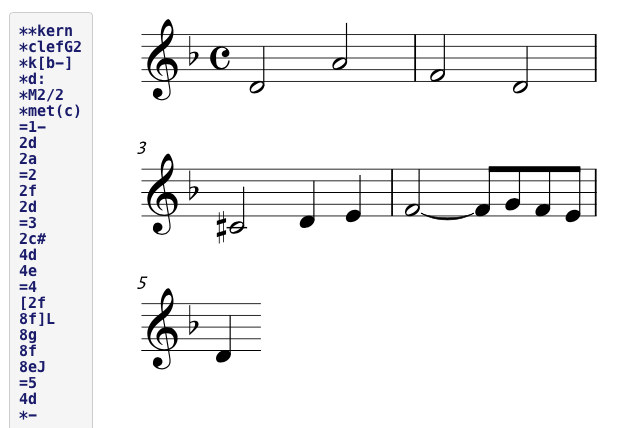
\includegraphics[scale=0.45]{imagesMem/humdrum.png}
        \caption{Representación de **kern}
    \end{figure}

    En esta representación podemos implementar notación moderna occidental además de poder manipular los siguientes apartados:

    \begin{itemize}
        \item El tono: alteraciones musicales, claves, posición de claves, armadura, fórmula de compás
        \item La duración: silencios, puntos, ligaduras, ligados.
        \item Articulaciones y ornamentos: staccato, tenuto, pizzicato.
    \end{itemize}

    Una variante de la representación **kern es **mens. Este tipo de representación acoge todo tipo de notación mensural blanca
    con muchas coincidencias con **kern a la hora de representarse, ya que este tipo de notación también es vertical y se gestiona
    de una forma muy parecida a la de notación moderna.

    El defecto que lleva a esta representación a no estar realmente completa es la falta de gramática que es el tema correspondiente
    a este trabajo y que explicaremos a continuación.

    \subsection{Decisiones sobre la gramática}
    Para poder implementar una gramática hay que hacer cierto balance de como va a ser la complejidad de esta y discutir
    de que manera puede ser la más correcta u óptima de realizarla.
    \subsubsection{Analizador sintáctico descendente o ascendente}
    Este puede ser un problema que suele suceder en estos casos, que tipo de analizador sintáctico elegir, ascendente o
    descendente.
    Como ya hemos explicado anteriormente con más detalle, un analizador sintáctico descendente genera el árbol de sintaxis
    desde el nodo inicial a las hojas (nodos terminales) derivando estos primeros nodos en reglas de producción compuestas
    de nodos terminales y nodos no terminales, mientras el analizador sintáctico ascendente genera este árbol de abajo hacia
    arriba, donde los nodos terminales se juntan creando reglas de producción has llegar al nodo inicial.

    Para la elección de que tipo de analizador vamos a escoger, debemos entender que ventajas e inconvenientes tiene cada
    uno. Por un lado, el analizador sintáctico ascendente es más eficiente a la hora de detección de errores respecto al
    descendente ya que va generando reglas conforme reconoce tokens hasta llegar al nodo raíz. Además, tiene
    un reconocimiento muy rápido, aunque no tanto como el descendente. Por otro lado, el analizador sintáctico descendente
    una gran ventaja reside en la facilidad de ser implementado, además, como ya hemos dicho, es un método de reconocimiento
    más rápido que el ascendente.

    Dadas las ventajas y desventajas que hemos anotado, también debemos exponer que herramienta nos conviene más, \textit{ANTLR}
    o \textit{flex/bison}, ya que serán las herramientas que necesitaremos para la creación de nuestra gramática.

    Bien, como sabemos, una gran diferencia que reside entre \textit{ANTLR} y \textit{flex/bison} es que son analizadores
    sintácticos descendentes y ascendentes, respectivamente. Otra gran diferencia entre ambos es el apartado que engloba
    cada una de estas herramientas, ya que con la primera podemos obtener mejor flexibilidad a la hora de creación del lenguaje
    que con \textit{flex/bison}, porque el primera engloba más fases de compilación que el segunda.

    \begin{figure}[H]
        \centering
        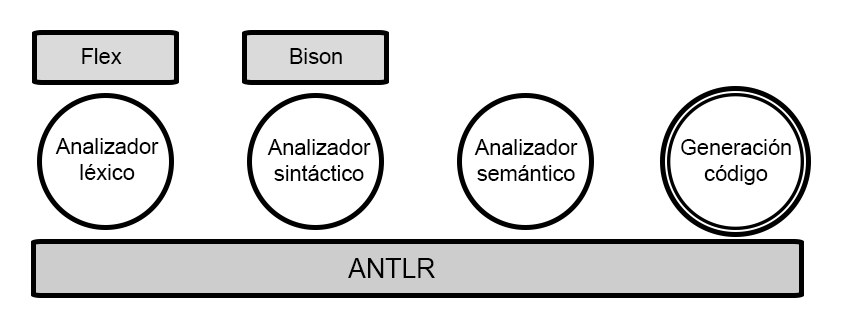
\includegraphics[scale = 0.6]{imagesMem/flexantlr.png}
        \caption{Comparación entre ANTLR y flex/bison}
    \end{figure}

    Sabiendo estos detalles que hemos explicado, la elección del formato de analización sintáctica descendente es la correcta
    para este trabajo, ya que la grán cantidad de \textit{tokens} y de reglas a formar hace que sea una gramática compleja,
    además la utilización de ANTLR puede provocar que en un futuro mejore la semántica de esta ya que será posible de implementar
    e incluso fabricar traductores a otros tipos de representación musical, como DARMS o SCORE por ejemplo.

    Además, ANTLR soporta el algoritmo de lenguaje EBFN, el cual es una extension del algoritmo BNF (\textit{Backus-Naur Form})
    que es la notación formal para definir la sintaxis de un lenguaje. EBNF soporta símbolos que simplifican las reglas de
    producción. Más adelante explicaremos como es la utilización de este algoritmo.

    \subsection{Notación de gramática.}
    Como ya hemos dicho nuestra gramática va a tener un tipo de notación EBNF, la cual es una extensión en BNF, lo que
    produce una simplificación de las reglas a implementar con el uso de diferentes símbolos.
    Para comprender la notación deberemos saber el uso de los diferentes símbolos.

    \begin{figure}[H]

                \texttt{numero ::=\space \space digito\space \space + ( '.' \space \space digito  + ) ? } \\
                \texttt{digito ::= '0' | '1' | '2' | '3' | '4' | '5' | '6' | '7' | '8' | '9'}

        \caption{Ejemplo de regla de gramática.}
    \end{figure}
    En la figura superior nos muestra un ejemplo de una regla de gramática con notación EBNF. Donde implementamos la gramática
    de un numero decimal o real.

    Como podemos observar hay diferentes símbolos que puede ser que no reconozcamos para la creación de la notación de una gramática:

    \begin{itemize}
        \item \texttt{::=} : este símbolo se utiliza para definir una regla atribuida a un nodo no terminal inicial, es decir:

        la regla ''numero'' derivará en (\texttt{digito\space \space + ( '.' \space \space digito  +})
        \item \texttt{?}: cuando utilizamos este símbolo significa que la regla puede tener o no el símbolo, regla o
        conjunto de estos. En nuestro ejemplo lo podemos observar englobando a todo lo que tenemos dentro del parentesis,
        esto querrá decir que la regla será valida aparezca o no los símbolos de dentro del parentesis.
        \item \texttt{+} o \texttt{*}: estos dos símbolos son utilizados para expresar que hay 1 o más, o ninguno o más
        símbolos, en nuestro caso podemos observar \texttt{+} lo que significa que habra al menos un \texttt{digito} inicial.
        \item \texttt{|}: es un símbolo para la representacion \textit{or} de una regla. En nuestro ejemplo lo podemos observar
        en la regla \texttt{digito} donde el resultado de esta puede ser cualquier número comprendido entre 0 y 9.
    \end{itemize}

    \subsection{Implementación de la gramática.}
    Una vez ya explicado los terminos necesarios para lograr entender como se puede realizar el trabajo, toca ver que
    metodología seguiremos para la implementación de esta gramática.

    \subsubsection{Metodología.}
    Dado a que nos guiaremos en la notación de Humdrum
    el método más eficiente en nuestro caso sera seguir una metodología de desarrollo guiado por pruebas el cual consiste
    en los siguientes pasos:
    \begin{itemize}
        \item Elegir un requisisto: Dado que podemos precisar de gran parte de la documentación de **kern y **mens podemos elegir
        cualquier requisito que deba soportar nuestra gramática.
        \item Escribir una prueba: Obtenido el requisito implementamos nuestra prueba unitaria con el fin de lograr resolverla.
        \item Verificar el fallo de la prueba: En caso de no fallar el requisito que hemos obtenido está paliado, mientras
        que si falla deberemos modificar las reglas para que supere la prueba correctamente.
        \item Escribir la implementación correcta: Modificación de la regla de manera correcta con el fin de que la prueba sea
        verificada correctamente.
        \item Ejecutar las conjunto de pruebas: Una vez superadas cada una de manera unitaria, deberemos ejecutar todas en
        su conjunto ya que al modificar unas puede haber repercutido en otras, si al llegar al fin no hemos logrado solucionarlo
        puede que necesitemos una refactorización de estas.
    \end{itemize}

    Este tipo de metodología requiere de unas reglas base y a partir de esta ir construyendo las diferentes reglas de producción
    que probaremos con los diferentes test.

    \subsection{Inicio y detalles}

    Nuestra gramática va a englobar tanto la notación **kern, como la notación **mens, es decir, vamos a poder implementar
    código con la finalidad de que nuestro analizador sintáctico descendente verifique que el código esta correctamente
    implementado.
    Dado en algunos aspectos ambas gramáticas son parecidas algunas de las reglas servirán para ambos tipos de notación,
    pudiendo compartirlas entre sí.

    Como punto de inicio tendremos una regla inicial, que denominamos en nuestro caso \texttt{startRule}, esta creará una
    bifurcación entre ambas notaciones (**kern y **mens).
    Cabe mencionar que en las reglas podremos visualizar dos estilos de símbolos los que estan entre comillas y los que no.
    Los primeros representarán a los nodos terminales mientras que los otros a los nodos no terminales.
    \begin{table}[H]
        \centering
        \texttt{startRule ::= kern\_notation + | mens\_notation +}
    \end{table}

    \begin{figure}[H]
        \centering
        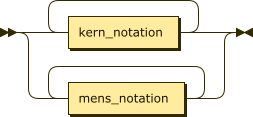
\includegraphics{figures_railroad/png/skern/startRule.png}
        \caption{Regla inicial}
    \end{figure}

    Como hemos dicho previamente y podemos observar esta regla crea la separación entre ambas notaciones dandole la importancia
    de la elección de una notación u otra, además una vez elegida podemos observar que no puede cambiar a la anterior, será
    o **kern o **mens.

    \subsection{**kern}
    Una vez elegida la notación a utilizar pasamos a explicar una de ellas, **kern, esta notación representa a la que utilizamos
    actualmente en música, la notación moderna occidental.

    Para ello debemos establecer una cabecera y un final que abarque a este tipo de notación y además la identifique como
    que es **kern:

    \begin{table}[H]
        \texttt{kern\_notation::= ''*'' ''*'' ''kern'' mastercleff keysignature ? timesignature ? musicalcontent ''*-''}
    \end{table}

    \begin{figure}[H]
    \centering
        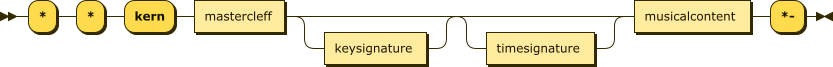
\includegraphics[scale = 0.55]{figures_railroad/png/skern/kern_notation.png}
        \caption{Regla que deriva a la notación **kern}
    \end{figure}

    Esta regla lo que conseguimos es realizar una división de lo que sería el pentagrama inicial en las cuatro piezas más
    básicas y fundamentales: clave, armadura de compás, tiempo de compás y el contenido musical.

    \begin{figure}[H]
        \centering
        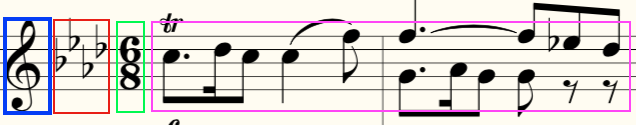
\includegraphics[scale = 0.5]{imagesMem/pentagrama.png}
        \caption{Representación de regla **kern}
    \end{figure}

    Como podemos observar en la figura anterior de una manera más visual, la regla inicial de **kern divide
    la clave que contendrá el pentagrama (azul), la armadura de dicho pentagrama (roja), el tiempo de compás que tendrá la composición (verde) y
    y el contenido musical (magenta), además algunas de estas partes puede que no nos las encontremos ya que no son imprescindibles
    en la notación.

    \subsection{Clave}
    Para este apartado, la regla es muy sencilla.

    \begin{figure}[H]
        \centering
        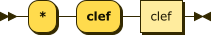
\includegraphics[scale = 0.55]{figures_railroad/png/skern/mastercleff.png}
        \caption{Representación de la clave del compás.}
    \end{figure}

    Dado un encabezado con \texttt{*clef} y una de las claves de nuestra notación podemos forma la clave de nuestros pentagrama.

    \subsection{Armadura de compás}
    La aplicación de la armadura del compás se realizará con un previo asterisco y entre corchetes los cuales contendrán
    las notas con sus sostenidos o bemoles.
    \begin{figure}[H]
        \centering
        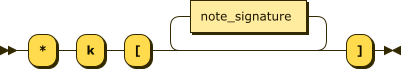
\includegraphics[scale = 0.55]{figures_railroad/png/skern/keysignature.png}
        \caption{Representación de armadura de compás.}
    \end{figure}

    \subsection{Tiempo de compás}
    La definimos con una fracción en la que puede haber una estructura rítmica que represente a un compas, como podría ser
    el \textit{compasillo}. Todo esto debe ir precedido con \texttt{*k}.
    \begin{figure}[H]
        \centering
        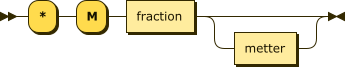
\includegraphics[scale = 0.55]{figures_railroad/png/skern/timesignature.png}
        \caption{Representación de tiempo de compás.}
    \end{figure}

    \subsection{Contenido de compás}
    Esto representa la parte más amplia de nuestra gramática en torno a la notación de **kern. En este apartado es donde
    tendremos gran parte de la representación musical: ritmo, notas, alteraciones...

%todo EMPIEZA LA BIBLIOGRAFIA (REFERENCIAS%
    \newpage
    \todo[inline]{como puede referenciar la bibliografia de alguien entonces?.}
    \begin{thebibliography}{9}
        \bibitem{babbage}
        \texttt{https://es.wikipedia.org/wiki/Charles\_Babbage}

        \bibitem{flex}
        Herramienta generadora de analizadores léxicos desarrollada por Robert P. Corbett alrededor de 1987.
        \texttt{https://github.com/westes/flex}

        \bibitem{bison}
        Herramienta generadora de analizadores sintácticos creada por Robert P. Corbett en junio de 1985.
        \texttt{http://www.gnu.org/software/bison/}


        \bibitem{antlr4}
        Terrence Par (2012), \textit{The Definitive ANTLR 4 Reference}. The Pragmatic Programmers, LLC.

        \bibitem{kern}
        Notación musical creada por David Huron en la decada de 1980.
        \texttt{https://www.humdrum.org/guide/ch02/}

        \bibitem{mens}
        Notación mensural blanca derivada de **kern
        \texttt{https://doc.verovio.humdrum.org/humdrum/mens/}

        \bibitem{darms}
        Digital Alternate Representation of Musical Scores creado en 1966 por Stefan Bauer-Mengelberg.

        \bibitem{score}
        Sistema de representación musical creado en 1971 por Leland Smith.

        \bibitem{esac}
        Sistema de representación desarrollado para crear música monofónica a finales de los 80s por Helmut Schaffrasth.

        \bibitem{humdrum}
        \texttt{https://www.humdrum.org}.




    \end{thebibliography}
\end{document}